\let\negmedspace\undefined
\let\negthickspace\undefined
%\RequirePackage{amsmath}
\documentclass[journal,12pt,twocolumn]{IEEEtran}
%
% \usepackage{setspace}
 \usepackage{gensymb}
%\doublespacing
%\singlespacing
%\usepackage{silence}
%Disable all warnings issued by latex starting with "You have..."
%\usepackage{graphicx}
\usepackage{amssymb}
%\usepackage{relsize}
\usepackage[cmex10]{amsmath}
%\usepackage{amsthm}
%\interdisplaylinepenalty=2500
%\savesymbol{iint}
%\usepackage{txfonts}
%\restoresymbol{TXF}{iint}
%\usepackage{wasysym}
\usepackage{amsthm}
%\usepackage{pifont}
%\usepackage{iithtlc}
% \usepackage{mathrsfs}
% \usepackage{txfonts}
 \usepackage{stfloats}
% \usepackage{steinmetz}
 \usepackage{bm}
% \usepackage{cite}
% \usepackage{cases}
% \usepackage{subfig}
%\usepackage{xtab}
\usepackage{longtable}
%\usepackage{multirow}
%\usepackage{algorithm}
%\usepackage{algpseudocode}
\usepackage{enumitem}
 \usepackage{mathtools}
 \usepackage{tikz}
% \usepackage{circuitikz}
% \usepackage{verbatim}
%\usepackage{tfrupee}
\usepackage[breaklinks=true]{hyperref}
%\usepackage{stmaryrd}
%\usepackage{tkz-euclide} % loads  TikZ and tkz-base
%\usetkzobj{all}
\usepackage{listings}
    \usepackage{color}                                            %%
    \usepackage{array}                                            %%
    \usepackage{longtable}                                        %%
    \usepackage{calc}                                             %%
    \usepackage{multirow}                                         %%
    \usepackage{hhline}                                           %%
    \usepackage{ifthen}                                           %%
  %optionally (for landscape tables embedded in another document): %%
    \usepackage{lscape}     
% \usepackage{multicol}
% \usepackage{chngcntr}
%\usepackage{enumerate}

%\usepackage{wasysym}
%\newcounter{MYtempeqncnt}
\DeclareMathOperator*{\Res}{Res}
\DeclareMathOperator*{\equals}{=}
%\renewcommand{\baselinestretch}{2}
\renewcommand\thesection{\arabic{section}}
\renewcommand\thesubsection{\thesection.\arabic{subsection}}
\renewcommand\thesubsubsection{\thesubsection.\arabic{subsubsection}}

\renewcommand\thesectiondis{\arabic{section}}
\renewcommand\thesubsectiondis{\thesectiondis.\arabic{subsection}}
\renewcommand\thesubsubsectiondis{\thesubsectiondis.\arabic{subsubsection}}

% correct bad hyphenation here
\hyphenation{op-tical net-works semi-conduc-tor}
\def\inputGnumericTable{}                                 %%

\lstset{
%language=C,
frame=single, 
breaklines=true,
columns=fullflexible
}
%\lstset{
%language=tex,
%frame=single, 
%breaklines=true
%}
\begin{document}

%


\newtheorem{theorem}{Theorem}[section]
\newtheorem{problem}{Problem}
\newtheorem{proposition}{Proposition}[section]
\newtheorem{lemma}{Lemma}[section]
\newtheorem{corollary}[theorem]{Corollary}
\newtheorem{example}{Example}[section]
\newtheorem{definition}[problem]{Definition}
%\newtheorem{thm}{Theorem}[section] 
%\newtheorem{defn}[thm]{Definition}
%\newtheorem{algorithm}{Algorithm}[section]
%\newtheorem{cor}{Corollary}
\newcommand{\BEQA}{\begin{eqnarray}}
\newcommand{\EEQA}{\end{eqnarray}}
\newcommand{\define}{\stackrel{\triangle}{=}}
\newcommand*\circled[1]{\tikz[baseline=(char.base)]{
    \node[shape=circle,draw,inner sep=2pt] (char) {#1};}}
\bibliographystyle{IEEEtran}
%\bibliographystyle{ieeetr}


\providecommand{\mbf}{\mathbf}
\providecommand{\pr}[1]{\ensuremath{\Pr\left(#1\right)}}
\providecommand{\qfunc}[1]{\ensuremath{Q\left(#1\right)}}
\providecommand{\sbrak}[1]{\ensuremath{{}\left[#1\right]}}
\providecommand{\lsbrak}[1]{\ensuremath{{}\left[#1\right.}}
\providecommand{\rsbrak}[1]{\ensuremath{{}\left.#1\right]}}
\providecommand{\brak}[1]{\ensuremath{\left(#1\right)}}
\providecommand{\lbrak}[1]{\ensuremath{\left(#1\right.}}
\providecommand{\rbrak}[1]{\ensuremath{\left.#1\right)}}
\providecommand{\cbrak}[1]{\ensuremath{\left\{#1\right\}}}
\providecommand{\lcbrak}[1]{\ensuremath{\left\{#1\right.}}
\providecommand{\rcbrak}[1]{\ensuremath{\left.#1\right\}}}
\theoremstyle{remark}
\newtheorem{rem}{Remark}
\newcommand{\sgn}{\mathop{\mathrm{sgn}}}
\providecommand{\abs}[1]{\left\vert#1\right\vert}
\providecommand{\res}[1]{\Res\displaylimits_{#1}} 
\providecommand{\norm}[1]{\left\lVert#1\right\rVert}
%\providecommand{\norm}[1]{\lVert#1\rVert}
\providecommand{\mtx}[1]{\mathbf{#1}}
\providecommand{\mean}[1]{E\left[ #1 \right]}
\providecommand{\fourier}{\overset{\mathcal{F}}{ \rightleftharpoons}}
%\providecommand{\hilbert}{\overset{\mathcal{H}}{ \rightleftharpoons}}
\providecommand{\system}{\overset{\mathcal{H}}{ \longleftrightarrow}}
	%\newcommand{\solution}[2]{\textbf{Solution:}{#1}}
\newcommand{\solution}{\noindent \textbf{Solution: }}
\newcommand{\cosec}{\,\text{cosec}\,}
\providecommand{\dec}[2]{\ensuremath{\overset{#1}{\underset{#2}{\gtrless}}}}
\newcommand{\myvec}[1]{\ensuremath{\begin{pmatrix}#1\end{pmatrix}}}
\newcommand{\mydet}[1]{\ensuremath{\begin{vmatrix}#1\end{vmatrix}}}
%\numberwithin{equation}{section}
\numberwithin{equation}{subsection}
%\numberwithin{problem}{section}
%\numberwithin{definition}{section}
\makeatletter
\@addtoreset{figure}{problem}
\makeatother

\let\StandardTheFigure\thefigure
\let\vec\mathbf
%\renewcommand{\thefigure}{\theproblem.\arabic{figure}}
\renewcommand{\thefigure}{\theproblem}
%\setlist[enumerate,1]{before=\renewcommand\theequation{\theenumi.\arabic{equation}}
%\counterwithin{equation}{enumi}


%\renewcommand{\theequation}{\arabic{subsection}.\arabic{equation}}

\def\putbox#1#2#3{\makebox[0in][l]{\makebox[#1][l]{}\raisebox{\baselineskip}[0in][0in]{\raisebox{#2}[0in][0in]{#3}}}}
     \def\rightbox#1{\makebox[0in][r]{#1}}
     \def\centbox#1{\makebox[0in]{#1}}
     \def\topbox#1{\raisebox{-\baselineskip}[0in][0in]{#1}}
     \def\midbox#1{\raisebox{-0.5\baselineskip}[0in][0in]{#1}}

\vspace{3cm}

\title{
	%\logo{
%Computational Approach to School Geometry
	Matrix Analysis
%	}
}
\author{ G V V Sharma$^{*}$% <-this % stops a space
	\thanks{*The author is with the Department
		of Electrical Engineering, Indian Institute of Technology, Hyderabad
		502285 India e-mail:  gadepall@iith.ac.in. All content in this manual is released under GNU GPL.  Free and open source.}
	
}	
%\title{
%	\logo{Matrix Analysis through Octave}{\begin{center}\includegraphics[scale=.24]{tlc}\end{center}}{}{HAMDSP}
%}


% paper title
% can use linebreaks \\ within to get better formatting as desired
%\title{Matrix Analysis through Octave}
%
%
% author names and IEEE memberships
% note positions of commas and nonbreaking spaces ( ~ ) LaTeX will not break
% a structure at a ~ so this keeps an author's name from being broken across
% two lines.
% use \thanks{} to gain access to the first footnote area
% a separate \thanks must be used for each paragraph as LaTeX2e's \thanks
% was not built to handle multiple paragraphs
%

%\author{<-this % stops a space
%\thanks{}}
%}
% note the % following the last \IEEEmembership and also \thanks - 
% these prevent an unwanted space from occurring between the last author name
% and the end of the author line. i.e., if you had this:
% 
% \author{....lastname \thanks{...} \thanks{...} }
%                     ^------------^------------^----Do not want these spaces!
%
% a space would be appended to the last name and could cause every name on that
% line to be shifted left slightly. This is one of those "LaTeX things". For
% instance, "\textbf{A} \textbf{B}" will typeset as "A B" not "AB". To get
% "AB" then you have to do: "\textbf{A}\textbf{B}"
% \thanks is no different in this regard, so shield the last } of each \thanks
% that ends a line with a % and do not let a space in before the next \thanks.
% Spaces after \IEEEmembership other than the last one are OK (and needed) as
% you are supposed to have spaces between the names. For what it is worth,
% this is a minor point as most people would not even notice if the said evil
% space somehow managed to creep in.

%\WarningFilter{latex}{LaTeX Warning: You have requested, on input line 117, version}


% The paper headers
%\markboth{Journal of \LaTeX\ Class Files,~Vol.~6, No.~1, January~2007}%
%{Shell \MakeLowercase{\textit{et al.}}: Bare Demo of IEEEtran.cls for Journals}
% The only time the second header will appear is for the odd numbered pages
% after the title page when using the twoside option.
% 
% *** Note that you probably will NOT want to include the author's ***
% *** name in the headers of peer review papers.                   ***
% You can use \ifCLASSOPTIONpeerreview for conditional compilation here if
% you desire.




% If you want to put a publisher's ID mark on the page you can do it like
% this:
%\IEEEpubid{0000--0000/00\$00.00~\copyright~2007 IEEE}
% Remember, if you use this you must call \IEEEpubidadjcol in the second
% column for its text to clear the IEEEpubid mark.



% make the title area
\maketitle

\newpage

\tableofcontents

\bigskip

\renewcommand{\thefigure}{\theenumi}
\renewcommand{\thetable}{\theenumi}
%\renewcommand{\theequation}{\theenumi}

%\begin{abstract}
%%\boldmath
%In this letter, an algorithm for evaluating the exact analytical bit error rate  (BER)  for the piecewise linear (PL) combiner for  multiple relays is presented. Previous results were available only for upto three relays. The algorithm is unique in the sense that  the actual mathematical expressions, that are prohibitively large, need not be explicitly obtained. The diversity gain due to multiple relays is shown through plots of the analytical BER, well supported by simulations. 
%
%\end{abstract}
% IEEEtran.cls defaults to using nonbold math in the Abstract.
% This preserves the distinction between vectors and scalars. However,
% if the journal you are submitting to favors bold math in the abstract,
% then you can use LaTeX's standard command \boldmath at the very start
% of the abstract to achieve this. Many IEEE journals frown on math
% in the abstract anyway.

% Note that keywords are not normally used for peerreview papers.
%\begin{IEEEkeywords}
%Cooperative diversity, decode and forward, piecewise linear
%\end{IEEEkeywords}



% For peer review papers, you can put extra information on the cover
% page as needed:
% \ifCLASSOPTIONpeerreview
% \begin{center} \bfseries EDICS Category: 3-BBND \end{center}
% \fi
%
% For peerreview papers, this IEEEtran command inserts a page break and
% creates the second title. It will be ignored for other modes.
%\IEEEpeerreviewmaketitle

\begin{abstract}
This manual provides an introduction to vectors and their properties,  based on the question papers, year 2020,  from Class 10 and 12, CBSE; JEE and JNTU.  
\end{abstract}








\section{Section A}
\begin{enumerate}[label=1.\arabic*]

\item The value(s) of k for which the quadratic equation $2x^2 + kx + 2 = 0$ has equal roots, is
\begin{enumerate}
    \item $4$
    \item $\pm 4$
    \item $- 4$\
    \item $0$
\end{enumerate}
\solution 
A quadratic equation 
		\begin{align}
			ax^2+bx + c  &= 0
		\end{align}
		has equal roots only if 
 the discriminant
		\begin{align}
			b^2 - 4a c  = 0
		\end{align}
		Substituting
		\begin{align}
			a = 2, b = k, c &= 2,
			\\
\implies 			k^2 - 4 &= 0
			\\
			\text{or, }k = \pm 4
		\end{align}

\item Which of the following is not an A.P. ?
\begin{enumerate}
    \item $-1.2, 0.8, 2.8...$
    \item $3, 3 + \sqrt{2}, 3 + 2\sqrt{2},3 + 3\sqrt{2}...$
    \item $\frac{4}{3}, \frac{7}{3}, \frac{9}{3}, \frac{12}{3}...$
    \item $\frac{-1}{5}, \frac{-2}{5}, \frac{-3}{5}$
\end{enumerate}
\solution $a_0, a_1, a_2$ can be terms of an AP only if 
		\begin{align}
	a_1 - 	a_0 = a_2 - 2a_1
		\end{align}
		Considering each of the above cases, 
		\begin{enumerate}
			\item 
				\begin{align}
					2.8 - 1.2 = 1.6 = 2(0.8)
				\end{align}
				Hence, the given terms are in A.P.
			\item 
				\begin{align}
					3 + \sqrt{2} - 3 = \sqrt{2} \\
					3 + 2\sqrt{2} - \brak{3+ \sqrt{2}}= \sqrt{2} \\
					3 + 3\sqrt{2} - \brak{3+ 2\sqrt{2}}= \sqrt{2} 
				\end{align}
				Hence, the given terms are in A.P.
    \item 
	    \begin{align}
		    \frac{7}{3} -   \frac{4}{3} &= 1
		    \\
		     \frac{9}{3}-\frac{7}{3} &= \frac{2}{3}
		     \\
		    \frac{12}{3}-\frac{9}{3} &= 1
	    \end{align}
				Hence, the given terms are not in A.P.
				\end{enumerate}

\item The radius of a sphere (in cm), whose volume is $12\pi cm^3$, is
\begin{enumerate}
    \item $3$
    \item $3 \sqrt{2}$
    \item $3^\frac{2}{3}$
    \item $3^\frac{1}{3}$
\end{enumerate}
\solution 
The volume of a sphere, given the radius $r$, is given by
\begin{align}
	V = \frac{4}{3}\pi r^3
\end{align}

\item The distance between the points (m , -n) and (-m , n) is
\begin{enumerate}
    \item $\sqrt{m^2 + n^2}$
    \item $m + n$
    \item $2\sqrt{m^2 + n^2}$
    \item $\sqrt{2m^2 + 2n^2}$
\end{enumerate}
		\solution Letting 
		\begin{align}
			\vec{A} &= \myvec{m \\ -n}, \vec{B}=\myvec{-m \\ n}
			\\
			\vec{A}-\vec{B} &= 2\myvec{m \\ -n}
		\end{align}
Using the definition   of the norm in \eqref{eq:norm2d},
		\begin{align}
\norm{\vec{A}-\vec{B}} &=2\norm{\myvec{m \\ -n}}
			\\
			&=2 \sqrt{\myvec{m & -n}\myvec{m \\ -n}} 
\\
			&			= 2 \sqrt{m^2+n^2}
		\end{align}

\item In Fig. $\ref{Fig1}$ ,from an external point P, two tangents $\Vec{PQ}$ and $\Vec{PR}$ are drawn to a circle of radius 4cm with center O. If $\angle{QPR} = 90\degree$, then length of $\Vec{PQ}$ is
\begin{enumerate}
    \item $3$
    \item $4$
    \item $2$
    \item $2\sqrt{2}$
\end{enumerate}
\solution In general, for a circle with radus $r$ and $\angle{QPR} = \theta$, 
\begin{align}
	PQ &= r \cot \frac{\theta}{2}
	\\
	&= 4 \cot 45 \degree = 4
\end{align}
upon substituting numerical values.
\begin{figure}[h!]
    \centering
    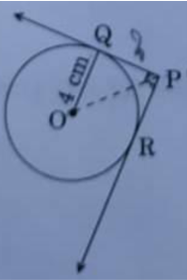
\includegraphics[width=0.5\columnwidth]{Fig1.png}
	\caption{}
	\label{Fig1}
 \end{figure}
 
 \item On dividing a polynomial p$\myvec{x}$ by $x^2 - 4$, the quotient and remainder are found to be x and 3 respectively. The polynomial p$\myvec{x}$
 \begin{enumerate}
    \item $3$
    \item $4$
    \item $2$
    \item $2\sqrt{2}$
\end{enumerate}
\solution In general, the polynomial
\begin{align}
	p(x) &= d(x)q(x) + r(x)
	\\
	&= \brak{x^2-4}x +3
	\\
	&= x^3 - 4x + 3
\end{align}
\item In Fig $\ref{Fig2}$ ,$DE \parallel BC$. If $\frac{AD}{DB} = \frac{3}{2}$ and $AE = 2.7cm$, then $EC$ is equal to 
\begin{enumerate}
    \item $2.0 cm$
    \item $1.8 cm$
    \item $4.0 cm$
    \item $2.7 cm$
\end{enumerate}
\solution Since 
\begin{align}
	\frac{AD}{DB}  &= 
	\frac{AE}{EC}
	\\
	\implies \frac{3}{2}&= \frac{2.7}{EC}
	\\
	\text{or, }
	EC & = 1.8
\end{align}

\begin{figure}[h!]
    \centering
    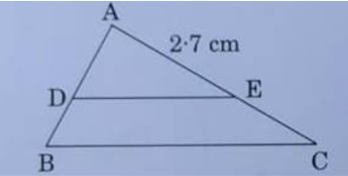
\includegraphics[width=0.5\columnwidth]{Fig2.png}
	\caption{}
	\label{Fig2}
 \end{figure}
 
\item \begin{enumerate}
\item The point on the x axis which is equidistant from $\myvec{-4 \\ 0}$ and $\myvec{10\\0}$\\
\begin{enumerate}
\item $\myvec{7,0}$
\item $\myvec{5,0}$
\item $\myvec{0,0}$
\item $\myvec{3,0}$
\end{enumerate}
\solution If $\vec{x}$ lies on the  $x$-axis and is  equidistant from the points $\vec{A}$ and $\vec{B}$, 
  \begin{align}
	  \vec{x} &=
	   x\vec{e}_1
  \end{align}
  where 
  \begin{align}
	  x &=\frac{\norm{\vec{A}}^2 -\norm{\vec{B}}^2 }{2\brak{\vec{A}-\vec{B}}^{\top }\vec{e}_1
}
	  &= 3
	  \label{eq:cbse_10_x}
  \end{align}
upon   substituting numerical values. 
  Hence, the desired point is $\myvec{ 3 \\ 0}$.

\item The center of a circle whose end points of a diameter are $\myvec{-6, 3}$ and $\myvec{6,4}$ is
\begin{enumerate}
\item $\myvec{8,-1}$
\item $\myvec{4,7}$
\item $\myvec{0,\frac{7}{2}}$
\item $\myvec{4,\frac{7}{2}}$
\end{enumerate}
		\solution 
Using section formula, 
		the desired point is given by 
  \begin{align}
	  \vec{O}&= \frac{\vec{B}+ \vec{A}}{2}
	  \\
	  &= \frac{1}{2}\sbrak{\myvec{ -6 \\ 3}+\myvec{6 \\ 4}}
	  \\
	  &=\frac{1}{2}\myvec{0 \\ 7}
  \end{align}
%    See Fig. 
%	  \ref{fig:cbse-10-3.pdf}
%  \begin{figure}
%	  \centering 
%	  \includegraphics[width=\columnwidth]{figs/cbse-10-3.pdf}
%	  \caption{}
%	  \label{fig:cbse-10-3.pdf}
%	  \end{figure}
\end{enumerate}

\item The pair of linear equations,
	\begin{align}
		\frac{3x}{2} + \frac{5y}{3} &=7  \text{ and}\\
		9x + 10y &= 14
	\end{align}
		is
\begin{enumerate}
\item consistent
\item inconsistent 
\item consistent with one solution
\item consistent with many solutions
\end{enumerate}
\solution  The given system can be expressed as the matrix equation
	\begin{align}
		\myvec{\frac{3}{2} & \frac{5}{3} 
		\\
9 & 10 
		}\vec{x}=\myvec{7  \\14}
	\end{align}
	The augmented matrix can be expressed as 
	\begin{align}
		\myvec{\frac{3}{2} & \frac{5}{3} & 7
		\\
		9 & 10 & 14
		}
		\\
		\xleftrightarrow[]{R_1 \leftarrow 6R_1}
		\myvec{9 & 10 & 42
		\\
		9 & 10 &14
		}
		\\
		\xleftrightarrow[]{R_2 \leftarrow R_1 - R_2}
		\myvec{9 & 10 & 42
		\\
		0 & 0 & 28
		}
	\end{align}
From the above, it is obvious that the rank of the coefficient matrix is not equal to the rank of the augmented matrix.  Hence, the system is inconsistent.	

\item In Fig $\ref{Fig3}$, $\myvec{PQ}$ is tangent to the circle with center at O, at the point B. If $\angle{AOB} = 100\degree$, then $\angle{ABP}$ is equal to
\begin{enumerate}
\item $50\degree$
\item $40\degree$
\item $60\degree$
\item $80\degree$
\end{enumerate}

\begin{figure}[h!]
    \centering
    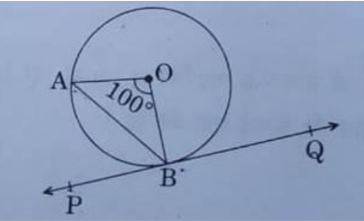
\includegraphics[width=0.5\columnwidth]{Fig3.png}
	\caption{}
	\label{Fig3}
 \end{figure}
 \solution  In general,
	\begin{align}
		\angle{ABP} &= \frac{1}{2} \angle{AOB} 
		\\
		&= 50 \degree
	\end{align}

 \end{enumerate}
\begin{enumerate}[label=2.\arabic*]
\item What is the simplest form of $\frac{1 + \tan^2 A}{1 + \cot^2 A}$\\
	\solution
		\begin{align}
			\frac{1 + \tan^2 A}{1 + \cot^2 A} 
			&=\frac{1 + \tan^2 A}{1 + \frac{1}{\tan^2 A}} 
			\\
			&=\tan^2 A
		\end{align}
	\item If the probablity of an event E happening is 0.023, then $P\brak{\bar{E}} = $\\
\item All concentric circles are \rule{1.5cm}{0.15mm} to each other\\

\item The probability of an event that is sure to happen is, \rule{1.5cm}{0.15mm}\\

\item AOBC is a rectangle whose 3 vertices are $A = \myvec{0,-3}$, $O = \myvec{0,0}$ and $B = \myvec{4,0}$. The length of the diagonal is \rule{1.5cm}{0.15mm}\\
\solution
The length of the diagonal is  
  \begin{align}
	  \norm{\vec{A}-\vec{B}} = \sqrt{3^2+4^2} = 5
  \end{align}

\item Write the value of $\sin^2 30\degree + \cos^2 60\degree$\\
	\solution Since 
  \begin{align}
	  \cos 60\degree &= \sin 30\degree, 
	  \\
	  \sin^2 30\degree + \cos^2 60\degree &= 
2\sin^2 30\degree 
\\
	  &=1
  \end{align}


\item \begin{enumerate}
    \item Form a quadratic polynomial, the sum and product of whose zeros are $\myvec{-3}$ and $2$ respectively.\\
	    \solution  The desired quadratic polynomial is 
  \begin{align}
	  \brak{x+3}\brak{x-2} = x^2-x-6
  \end{align}
    \item Can $\myvec{x^2 - 1}$ be a remainder while dividing $x^4 - 3x^2 + 5x - 9$ by $\myvec{x^2 + 3}$? ustify the reasons.\\
	    \solution  If the given statement be true, 
  \begin{align}
	  \frac{x^4 - 3x^2 + 5x - 9}{x^2 + 3} &= q(x) +\frac{ x^2 - 1}{x^2+3}
	  \\
	  &= q(x) +\frac{ x^2 +3 - 4}{x^2+3}
	  \\
	  &=q(x) + 1 - \frac{4}{x^2+3} 
  \end{align}
  which implies that the remainder is -4 resulting in a contradiction.  Hence, the given statement is not true.
\end{enumerate}

\item Find the sum of the first 100 natural numbers.\\
	\solution The sum of the first $n$ natural number is 
  \begin{align}
	  \frac{n\brak{n+1}}{2}
  \end{align}
Sustituting $n = 100$ in the above, the desired sum is 
  \begin{align}
50 \times 51 = 2550	
  \end{align}
\item The LCM of 2 numbers is 182 and their HCF is 13. If one of the numbers is 26, find the other.\\
\solution The desired number is obtained as
  \begin{align}
	  \frac{182 \times 13}{26} = 91
  \end{align}
\item In Fig $\ref{Fig4}$ the angle of elevation from the top of a tower from a point C on the ground, which is 30m away from the foot of the tower is $30\degree$. Find the height of the tower.\\
	\solution In general, the height is given by 
  \begin{align}
	  h &= d \tan \theta
	  \\
	  &= 30 \tan 30 \degree = 30 \frac{1}{\sqrt{3}}
	  \\
	  &= 10 \sqrt{3}
  \end{align}

\begin{figure}[h!]
    \centering
    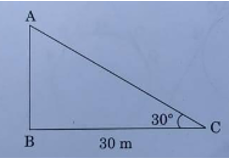
\includegraphics[width=0.5\columnwidth]{Fig4.png}
	\caption{}
	\label{Fig4}
 \end{figure}
\end{enumerate}


\section{Section B}
\begin{enumerate}[label=3.\arabic*]
    \item A cone and a cylinder have the same radii, but the height of the cone is 3 times that of the cylinder. Find the ratio of their volumes\\
   \solution Let $h_i, V_i, i = 1,2$ be the respective heights and volumes of the cone and the cylinder. 
   Then 
  \begin{align}
	  V_1 &= \frac{1}{3} \pi r^2 h_1
	  \\
	  V_2 &=  \pi r^2 h_2
	  \\
	  \implies \frac{V_1}{V_2} &= \frac{h_1}{3h_2}
	  \\
	  &= 1
  \end{align}
  $\because h_1 = 3h_2$.
    \item \begin{enumerate} 
    \item In Fig $\ref{Fig5}$, a quadrilateral ABCD is drawn to circumscribe a circle. Prove that $\vec{AB} + \vec{CD} = \vec{BC} + \vec{AD}$.\\
	    \solution 
    \begin{figure}[h!]
        \centering
        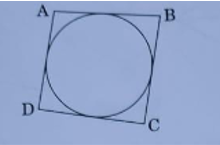
\includegraphics[width=0.5\columnwidth]{Fig5.png}
    	\caption{}
    	\label{Fig5}
     \end{figure}
     \item In Fig $\ref{Fig6}$, find the perimeter of $\triangle ABC$ if $\vec{AP} = 12cm$\\
    \begin{figure}[h!]
        \centering
        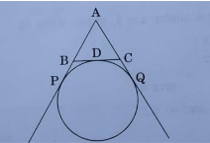
\includegraphics[width=0.5\columnwidth]{Fig6.png}
    	\caption{}
    	\label{Fig6}
     \end{figure}
     \end{enumerate}
      
     \item Find the mode of the following distribution:\\
     \vspace{2mm}\\
     \scalebox{0.7}{
     \begin{tabular}{|l|c|c|c|c|c|c|}
        \hline
        Marks & 0-10 & 10-20 & 20-30 & 30-40 & 40-50 & 50-60  \\
        \hline
        Number of Students  & 4 & 6 & 7 & 12 & 5 & 6\\
        \hline
     \end{tabular}
     }
     \vspace{2mm}
     
    \item In Fig $\ref{Fig7}$ if $\vec{PQ} \parallel \vec{BC}$ and $\vec{PR} \parallel \vec{CD}$, prove that $\frac{QB}{AQ} = \frac{DR}{AR}$.\\
    \begin{figure}[h!]
        \centering
        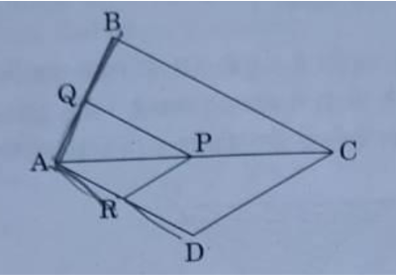
\includegraphics[width=0.5\columnwidth]{Fig7.png}
    	\caption{}
    	\label{Fig7}
     \end{figure}
    
    \item 
    \begin{enumerate}
        \item Show that $5 + 2\sqrt{7}$ is an irrational number, where $\sqrt{7}$ is given to be an irrational number.\\
        \item Check whether $12^n$ can end with the digit 0 for any natural number n.\\
		\solution  If $12^n$ ends with the digit 0, 
		    \begin{align}
			    12^{n} \equiv 0 {\pmod{10}}
		    \end{align}
		    However, 
		    \begin{align}
			    12^{n} \not\equiv 0 {\pmod{10}}
		    \end{align}


		    it should be divisible by 10.  12 is not divisible by 10, neither is $12^2$.  Let us assume that $12^{n-1}$ is not divisible by 12.  Then, 
		    \begin{align}
			    12^{n} = 12.12^{n-1}
		    \end{align}
		    Since neither 12 nor $12^{n-1}$ are divisible by 10, $12^{n}$ is also not divisible by $n$.
    \end{enumerate}
    
    \item If A, B and C are interior angles of $\triangle ABC$, then show that
		    \begin{align}
			    \label{eq:cbse-2020-10-tri}
    \cos \myvec{\frac{B + C}{2}} = \sin \myvec{\frac{A}{2}}
		    \end{align}
		    \solution In a triangle,
		    \begin{align}
			    A+B+C &= 180\degree
			    \\
			    \implies \myvec{\frac{B + C}{2}} &= 90\degree-\frac{A}{2}
			    \\
			    \text{or, }    \cos \myvec{\frac{B + C}{2}} = \sin \myvec{90\degree -\frac{A}{2}}
		    \end{align}
			    yielding \eqref{eq:cbse-2020-10-tri}.

\section{Section C}
    \item Prove that:\\
    $\myvec{\sin^4 - \cos^4 + 1} \csc^2\theta = 2$\\
    
    \item Find the sum:\\
    $\myvec{-5} + \myvec{-8} + \myvec{-11} + ... + \myvec{-230}$\\
    
    \item 
    \begin{enumerate}
    \item Construct a $\triangle ABC$ with sides $\vec{BC}=6cm$, $\vec{AB} = 5cm$ and $\angle{ABC} = 60\degree$. Then construct a triangle whose sides are $\frac{3}{4}$ of the corresponding sides of $\triangle ABC$.\\
    
    \item Draw a circle of radius $3.5 cm$. Take a point P outside the circle at a distance of $7 cm$ from the centre of the circle and construct a pair of tangents to the circle from that point. \\
    \end{enumerate}
    
    \item In Fig $\ref{Fig8}$, ABCD is a parallelogram. A semicircle with centre O and the diameter AB has been drawn and it passes through D. If $\Vec{AB} = 12$ and $\Vec{OD} \perp \Vec{AB}$, then find the area of the shaded region. Use $\myvec{\pi = 3.14}$\\
    \begin{figure}[h!]
        \centering
        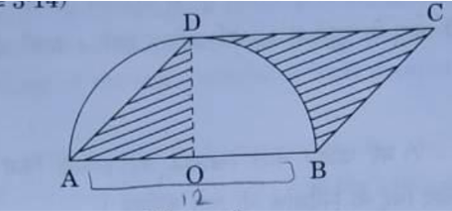
\includegraphics[width=0.5\columnwidth]{Fig8.png}
    	\caption{}
    	\label{Fig8}
     \end{figure} 
\end{enumerate}
\begin{enumerate}[label=4.\arabic*]
    \item A game in a booth at a Diwali Fair involves using a spinner first. Then, if the spinner stops on an even number, the player is allowed to pick a marble from a bag. The spinner and the marbles in the bag are represented in Fig $\ref{Fig9}$.\\
    Prizes are given, when a black marble is picked. Shweta plays the game once.
    \begin{figure}[h!]
        \centering
        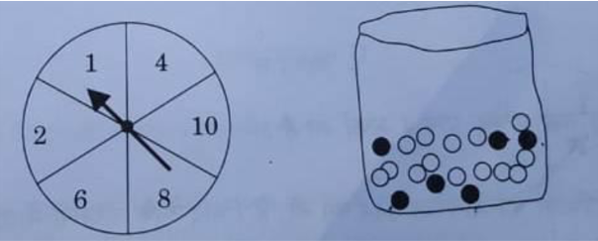
\includegraphics[width=0.5\columnwidth]{Fig9.png}
	    \caption{}
	    \label{Fig9}
    \end{figure} 
    \begin{enumerate}
        \item What is the probability that she will be allowed to pick a marble from the bag?\\
        \item Suppose she is allowed to pick a marble from the bag, what is the probability of getting a prize, when it is given that the bag contains 20 balls out of which 6 are black?\\
    \end{enumerate}
    \item \begin{enumerate}
        \item A fraction becomes $\frac{1}{3}$ when 1 is subtracted from the numerator and it becomes $\frac{1}{4}$ when 8 added to its denominator. Find the fraction.\\
        \item The present age of a father is three years more than three times the age of his son. Three years hence the father's age will be 10 years more than twice the age of the son. Determine their present ages.\\
    \end{enumerate} 
    \item \begin{enumerate}
        \item Find the ratio in which the y-axis divides the line segment joining the points $\myvec{6, -4}$ and $\myvec{-2, -7}$. Also find the point of intersection\\
\solution  In general, letting the given points be $\vec{A}, \vec{B}$, 
		\begin{align}
			\vec{P} &= \frac{k\vec{B}+ \vec{A} }{k+1}
			\label{eq:cbse-10-5-section}
		\end{align}
		Since the point lies on the $y$-axis, 
		\begin{align}
			\vec{e}_1^{\top}\vec{P} &= 0
			\\
			\implies k\vec{e}_1^{\top}\vec{B}+ \vec{e}_1^{\top}\vec{A} &=0
			\\
			\text{or, } k &=- \frac{\vec{e}_1^{\top}\vec{A}}{\vec{e}_1^{\top}\vec{B}}
		\end{align}
Substituting in 			\eqref{eq:cbse-10-5-section} and simplifying, 
		\begin{align}
			\vec{P} &= \frac{\brak{\vec{e}_1^{\top}\vec{B}}\vec{A}- \brak{\vec{e}_1^{\top}\vec{A}}\vec{B} }{\brak{\vec{e}_1^{\top}\vec{B}}-\brak{\vec{e}_1^{\top}\vec{A}}}
		\end{align}
        \item Show that the points $\myvec{7, 10}$, $\myvec{-2,5}$ and $\myvec{3, -4}$ and vertices of an isosceles right triangle.
		\\
		\solution Let the given points be $\vec{A}, \vec{B}, \vec{C}$ respectively. 
			 Then, the direction vectors of $AB, BC$ and $CA$ are
		\begin{align}
			\vec{A} -\vec{B}&= \myvec{7 \\ 10} -\myvec{-2 \\ 5} = \myvec{9 \\ 5}
			\\
			\vec{B} -\vec{C}&=  -\myvec{-2 \\ 5}-\myvec{3 \\ -4} = \myvec{-5 \\ 9}
			\\
			\vec{C} -\vec{A}&= \myvec{3 \\ -4} -\myvec{7 \\ 10} = \myvec{-4 \\ -14}
		\end{align}
		From the above,  we find that 
		\begin{align}
			\brak{\vec{A} -\vec{B}}^{\top}\brak{\vec{B} -\vec{C}}&=  \myvec{9 & 5}\myvec{-5 \\ 9}
			\\
			&=0
			\\
			\brak{\vec{B} -\vec{C}}^{\top}\brak{\vec{C} -\vec{A}}&=  \myvec{-5 & 9}\myvec{-4 \\ -14}
\\
			&=-106
			\\
			\brak{\vec{C} -\vec{A}}^{\top}\brak{\vec{A} -\vec{B}}&=  \myvec{-4 & -14}\myvec{9 \\ 5}
\\
			&=-106
		\end{align}
		From  the above equations, 
    \eqref{eq:angle2d} and 
    \eqref{eq:angle2d_orth},
		\begin{align}
			\brak{\vec{A} -\vec{B}}\perp \brak{\vec{B} -\vec{C}}
			\\
			\angle BCA = 
			\angle CAB  
		\end{align}
		Thus, the triangle is right angled and isosceles.
   \end{enumerate}
    \item Use Euclid Division Lemma to show that the square of any positive integer is either in the form $3q$ or $3q + 1$ for some integer q.\\
\section{Section D}
    \item \begin{enumerate}
        \item Sum of the areas of two squares is $544 m^2$. If the difference of their perimeters is $32m$, find the sides of the two squares.\\
        \item A motorboat whose speed is 18 kmph in still water takes 1 hour more to go 24 km upstream than to return downstream than to return downstream to the same spot. Find the speed of the stream.\\
    \end{enumerate}
    \item \begin{enumerate}
        \item For the following data, draw a 'less than' ogive and hence find the median of the distribution.\\
     \vspace{2mm}\\
     \scalebox{0.6}{
    \begin{tabular}{|l|c|c|c|c|c|c|c|}
        \hline
        Age & 0-10 & 10-20 & 20-30 & 30-40 & 40-50 & 50-60 & 60-70  \\
        \hline
        Number of people & 5 & 15 & 20 & 25 & 15 & 11 & 9\\
        \hline
    \end{tabular}
    }
    \vspace{2mm}\\
    \item The distribution given below shows the number of wickets taken by bowlers in one-day cricket matches. Find the mean and the median of the number of wickets. Find the mean and the median of the number of wickets taken.\\
     \vspace{2mm}\\
     \scalebox{0.6}{
    \begin{tabular}{|l|c|c|c|c|c|c|c|}
        \hline
        Number of wickets & 0-10 & 10-20 & 20-30 & 30-40 & 40-50 & 50-60 & 60-70  \\
        \hline
        Number of bowlers & 5 & 15 & 20 & 25 & 15 & 11 & 9\\
        \hline
    \end{tabular}
    }    
    \vspace{2mm}\\
    \end{enumerate}
    \item A statue $1.6m$ tall, stands on the top of a pedestal. From a point on the ground,  the angle of elevation of the top of the statue is $60\degree$ and from the same point the angle of elevation of the top of the pedestal is $45\degree$. Find the height of the pedestal.Use$\myvec{\sqrt{3} = 1.73}$\\
    
    \item \begin{enumerate}
        \item  Obtain other zeros of the polynomial\\
    $p \myvec{x} = 2x^4 - x^3 - 11x^2 + 5x + 5$\\
    if the two of its zeros are $\sqrt{5}$ and $- \sqrt{5}$\\
        \item What minimum must be added to $2x^3 - 3x^2 + 6x + 7$ so that the resulting polynomial will be divisible by $x^2 - 4x + 8$ ?\\
    \end{enumerate}
    
    \item In a cylindrical vessel of radius 10cm, containing some water, 9000 small spherical balls are dropped which are completely immersed in water which raises the water level. If each spherical ball is of radius 0.5 cm then find the rise in the level of water in the vessel.\\
    
    \item If a line is drawn parallel to one side of a triangle to intersect the other two sides at distinct points, prove that the other two sides are divided in the same ratio.\\
    
\end{enumerate}
\end{document}
